\documentclass[a4paper,11pt]{book}
\usepackage[T1]{fontenc}
\usepackage[utf8]{inputenc}
\usepackage{nicefrac,amssymb,amsthm,amsfonts,amsmath,epsfig,color,bm,yfonts,isomath}
\usepackage{tikz}
\usetikzlibrary{calc}

\begin{document}

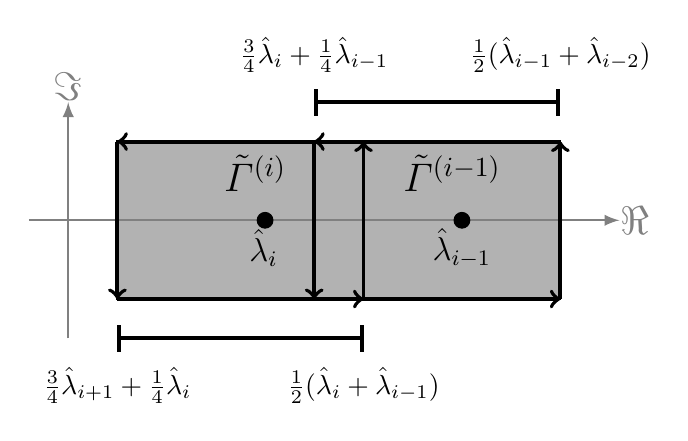
\begin{tikzpicture}
\coordinate (reAxisMin) at (-3,0);
\coordinate (reAxisMax) at (4.5,0);
\coordinate (imAxisMin) at (-2.5,-1.5);
\coordinate (imAxisMax) at (-2.5,1.5);
\coordinate (aLeft) at (-1.875,0);
\coordinate (aRight) at (1.25,0);
\coordinate (pLeft) at (0.624,0);
\coordinate (pRight) at (3.75,0);
\coordinate (aLambda) at (0,0);
\coordinate (pLambda) at (2.5,0);
\filldraw [thick, fill=gray!60, even odd rule] ($(aLeft)-(0,1)$)  coordinate (GeneralStart) -- ($(aRight)-(0,1)$) -- ($(aRight)+(0,1)$) -- ($(aLeft)+(0,1)$) -- cycle;
\filldraw [thick, fill=gray!60, even odd rule] ($(pLeft)-(0,1)$)  coordinate (GeneralStart) -- ($(pRight)-(0,1)$) -- ($(pRight)+(0,1)$) -- ($(pLeft)+(0,1)$) -- cycle;
\draw [line width=0.3mm, gray,-latex] (reAxisMin) -- (reAxisMax);% Draw x axis
\draw [line width=0.3mm, gray,-latex] (imAxisMin) -- (imAxisMax);% Draw y axis
\draw[->,line width=0.5mm] ($(aLeft)-(0,1)$) -- ($(aRight)-(0,1)$);
\draw[->,line width=0.5mm] ($(aRight)-(0,1)$) -- ($(aRight)+(0,1)$);
\draw[->,line width=0.5mm] ($(aRight)+(0,1)$) -- ($(aLeft)+(0,1)$);
\draw[->,line width=0.5mm] ($(aLeft)+(0,1)$) -- ($(aLeft)-(0,1)$);
\draw[->,line width=0.5mm] ($(pLeft)-(0,1)$) -- ($(pRight)-(0,1)$);
\draw[->,line width=0.5mm] ($(pRight)-(0,1)$) -- ($(pRight)+(0,1)$);
\draw[->,line width=0.5mm] ($(pRight)+(0,1)$) -- ($(pLeft)+(0,1)$);
\draw[->,line width=0.5mm] ($(pLeft)+(0,1)$) -- ($(pLeft)-(0,1)$);
\draw[|-|,line width=0.5mm] ($(aLeft)-(0,1.5)$) -- ($(aRight)-(0,1.5)$);
\draw[|-|,line width=0.5mm] ($(pLeft)+(0,1.5)$) -- ($(pRight)+(0,1.5)$);
\node[draw,circle,inner sep=2pt,fill] at (aLambda) {};
\node[draw,circle,inner sep=2pt,fill] at (pLambda) {};
\node at ($(aLambda)+(-0.02,-0.35)$) {\large $\hat\lambda_i$};
\node at ($(pLambda)+(0.0,-0.35)$) {\large $\hat\lambda_{i-1}$};
\node at ($(aLambda)+(-0.125,0.6)$) {\Large \textbf{$\tilde\Gamma^{(i)}$}};
\node at ($(pLambda)+(-0.125,0.6)$) {\Large \textbf{$\tilde\Gamma^{(i-1)}$}};
\node at ($(aLeft)-(0,2.1)$) {$\tfrac{3}{4} \hat\lambda_{i+1} + \tfrac{1}{4}\hat\lambda_i$};
\node at ($(aRight)-(0,2.1)$) {$\tfrac{1}{2} (\hat\lambda_{i} + \hat\lambda_{i-1})$};
\node at ($(pLeft)+(0,2.1)$) {$\tfrac{3}{4} \hat\lambda_{i} + \tfrac{1}{4}\hat\lambda_{i-1}$};
\node at ($(pRight)+(0,2.1)$) {$\tfrac{1}{2} (\hat\lambda_{i-1} + \hat\lambda_{i-2})$};
\node[gray] at ($(reAxisMax)+(0.2,0.0)$) {\Large $\Re$};
\node[gray] at ($(imAxisMax)+(0.0,0.2)$) {\Large $\Im$};
\end{tikzpicture}

\end{document}